\documentclass[11pt,a4paper,openany]{book}
\usepackage[margin=2.5cm]{geometry}
\usepackage{fontspec}
\usepackage{polyglossia}
\setmainlanguage{portuguese}
\usepackage{amsmath,amssymb,amsthm,mathtools}
\usepackage{unicode-math}
\setmainfont{Latin Modern Roman}
\setsansfont{Latin Modern Sans}
\setmonofont{Latin Modern Mono}[Scale=0.95]
\setmathfont{Latin Modern Math}
\usepackage{microtype}
\usepackage{booktabs,array,longtable}
\usepackage{graphicx}
\usepackage{xcolor}
\usepackage[most]{tcolorbox}
\usepackage{enumitem}
\usepackage{titlesec}
\usepackage{fancyhdr}
\usepackage[hidelinks]{hyperref}
\usepackage{setspace}
\raggedright
\setlength{\parindent}{0pt}
\setlength{\parskip}{0.7em}
\setstretch{1.1}
\emergencystretch=3em

\definecolor{azul}{HTML}{1F4E79}
\definecolor{verde}{HTML}{2E7D32}
\definecolor{laranja}{HTML}{B85C00}
\definecolor{cinza}{HTML}{F4F6F8}

\titleformat{\chapter}[display]{\bfseries\sffamily\color{azul}}{\Large Capítulo \thechapter}{0.4em}{\Huge}
\titlespacing*{\chapter}{0pt}{-10pt}{22pt}
\titleformat{\section}{\Large\bfseries\sffamily\color{azul}}{\thesection}{0.6em}{}
\titleformat{\subsection}{\large\bfseries\sffamily}{\thesubsection}{0.6em}{}

\pagestyle{fancy}
\fancyhf{}
\setlength{\headheight}{14pt}
\fancyhead[LE]{\small\sffamily\leftmark}
\fancyhead[RO]{\small\sffamily Guia de Econometria e Séries Temporais}
\fancyfoot[C]{\small\thepage}
\renewcommand{\headrulewidth}{0.3pt}

\newtcolorbox{intuicao}[1][Intuição]{colback=azul!5,colframe=azul,fonttitle=\bfseries\sffamily,title=#1,breakable,boxrule=0.6pt,arc=2pt}
\newtcolorbox{atencao}[1][Armadilha]{colback=laranja!7,colframe=laranja,fonttitle=\bfseries\sffamily,title=#1,breakable,boxrule=0.6pt,arc=2pt}
\newtcolorbox{simulacao}[1][Conferido por simulação]{colback=verde!6,colframe=verde,fonttitle=\bfseries\sffamily,title=#1,breakable,boxrule=0.6pt,arc=2pt}
\newtcolorbox{resumo}[1][Em uma página]{colback=cinza,colframe=black!60,fonttitle=\bfseries\sffamily,title=#1,breakable,boxrule=0.6pt,arc=2pt}

\newtheoremstyle{guia}{0.6em}{0.6em}{\itshape}{}{\bfseries\sffamily}{.}{0.5em}{}
\theoremstyle{guia}
\newtheorem{resultado}{Resultado}[chapter]
\theoremstyle{definition}
\newtheorem{exercicio}{Exercício}[chapter]

\newcommand{\E}{\mathbb{E}}
\newcommand{\Var}{\operatorname{Var}}
\newcommand{\Cov}{\operatorname{Cov}}
\newcommand{\plim}{\operatorname{plim}}
\newcommand{\bb}{\boldsymbol}
\newcommand{\sol}[1]{\textbf{Solução.} #1}

\begin{document}
\frontmatter
\begin{titlepage}
\centering
\vspace*{3cm}
{\sffamily\bfseries\color{azul}\fontsize{28}{34}\selectfont Guia de Econometria\\e Séries Temporais\par}
\vspace{1cm}
{\sffamily\Large Corte transversal, painel, séries temporais,\\volatilidade e aprendizado de máquina\par}
\vspace{2cm}
{\large Material de estudo em português, com explicações originais,\\experimentos numéricos conferidos e exercícios resolvidos\par}
\vfill
{\small Livros de referência para aprofundamento: Wooldridge, Goldberger, Stachurski, Hanck et al.,\\Hamilton, Lütkepohl, Cryer e Chan, Cowpertwait e Metcalfe, Mills, Tsay, Montgomery et al.,\\Hang Chan, Hastie et al., Faloutsos et al., Faouzi e Janati.}
\end{titlepage}
\tableofcontents
\mainmatter
\chapter*{Antes de começar}
\addcontentsline{toc}{chapter}{Antes de começar}
\markboth{Antes de começar}{Antes de começar}

Este guia foi escrito do zero, em português, com explicações próprias, para você aprender econometria de corte transversal, dados em painel e séries temporais. Ele \emph{não} é uma tradução de nenhum dos livros. Os livros enviados são a base de leitura aprofundada. Este material é o caminho didático para chegar até eles.

\section*{Como o guia está organizado}
Cada capítulo segue a mesma ordem: a ideia em linguagem simples, a matemática essencial, um experimento numérico que confirma a teoria, as armadilhas mais comuns e exercícios com solução. As caixas coloridas têm função fixa:

\begin{intuicao}[{Intuição}]
Explica o \emph{porquê} antes da fórmula.
\end{intuicao}
\begin{atencao}[{Armadilha}]
Erros frequentes, inclusive os que aparecem em livros e em manuais de software.
\end{atencao}
\begin{simulacao}[{Conferido por simulação}]
Resultado que eu rodei no computador (Python) para ter certeza de que a afirmação está correta. Os números são de uma semente fixa, então variam um pouco se você repetir.
\end{simulacao}

\section*{Mapa dos livros: onde aprofundar cada tema}
\begin{center}
\small
\begin{tabular}{p{4.3cm}p{9.6cm}}
\toprule
\textbf{Tema} & \textbf{Onde ler mais} \\
\midrule
Probabilidade e álgebra linear de base & Stachurski (\emph{Econometric Theory}, notas de curso), partes I e II; Goldberger \\
Regressão, MQO, VI & Wooldridge (cap. 4 e 5 da 1ª edição); Hanck et al. (cap. 4 a 9 e 12) \\
Dados em painel & Wooldridge (cap. 10 e 11); Hanck et al. (cap. 10) \\
ARMA, ARIMA, Box--Jenkins & Cryer e Chan (cap. 4 a 9); Mills (cap. 3, 4 e 7); Hamilton (cap. 3 e 4) \\
Raízes unitárias e cointegração & Hamilton (cap. 17 a 19); Mills (cap. 14); Hanck et al. (cap. 14 e 16) \\
VAR & Lütkepohl (\emph{New Introduction to Multiple Time Series Analysis}); Hamilton (cap. 11); Mills (cap. 13) \\
Volatilidade (ARCH/GARCH) & Tsay (\emph{Analysis of Financial Time Series}); Mills (cap. 10); Hamilton (cap. 21) \\
Aprendizado de máquina & Hastie, Tibshirani e Friedman (\emph{Elements of Statistical Learning}); tutorial de Faloutsos et al. sobre previsão em larga escala; Faouzi e Janati (pacote \texttt{pyts}) \\
\bottomrule
\end{tabular}
\end{center}

\section*{Duas observações sobre os livros}
\textbf{Edição do Wooldridge.} O arquivo que você enviou é a 1ª edição de \emph{Econometric Analysis of Cross Section and Panel Data} (2002, com impressão de 2004). Existe uma 2ª edição, de 2010, bem mais extensa. Os conceitos que uso aqui (MQO, VI, efeitos fixos e aleatórios) estão nas duas, mas a numeração de capítulos e alguns tópicos avançados mudam. Para o trabalho aplicado atual, vale ter a 2ª edição.

\textbf{Sobre ``corrigir os erros dos livros''.} Eu não auditei milhares de páginas atrás de erratas, e não vou fingir que sim. O que fiz foi (i) conferir por simulação toda fórmula e todo número que aparece neste guia e (ii) destacar, na caixa \emph{Armadilha}, os pontos onde os livros divergem entre si ou onde um erro é comum. O mais importante deles é o sinal do coeficiente de médias móveis, que muda de livro para livro (capítulo~\ref{cap:est}). Também não li os livros por inteiro: usei os sumários para montar o mapa acima e conferi diretamente em Cryer--Chan e em Mills a convenção de sinal do MA. Se você encontrar algo que não bate com seu livro, confie na simulação e na derivação, não no meu texto.

\section*{Notação}
Vetores e matrizes em negrito quando for útil. $\E(\cdot)$ é esperança, $\Var$ variância, $\Cov$ covariância, $\plim$ limite em probabilidade. $\hat\beta$ é um estimador e $\beta$ o parâmetro verdadeiro. Em séries temporais, $B$ é o operador de defasagem: $B y_t = y_{t-1}$.

\part{Fundamentos}
\chapter{Esperança condicional e projeção linear}
\label{cap:ec}

\section{Para que serve a esperança condicional}
Quase toda a econometria tenta responder: \emph{dado o que sei sobre $x$, qual é o valor típico de $y$?} A resposta matemática é a esperança condicional $m(x)=\E(y\mid x)$.

\begin{intuicao}
Imagine separar as pessoas por anos de estudo ($x$) e calcular o salário médio de cada grupo ($y$). A lista desses salários médios, um por grupo, é $m(x)$. Ela não diz nada sobre causa. Diz apenas qual é o salário médio de quem tem aquela escolaridade.
\end{intuicao}

\begin{resultado}[A esperança condicional é o melhor preditor]
Para qualquer função $g(x)$,
\[
\E\big[(y-g(x))^2\big] \;=\; \E\big[(y-m(x))^2\big] \;+\; \E\big[(m(x)-g(x))^2\big] \;\ge\; \E\big[(y-m(x))^2\big].
\]
Logo $m(x)$ minimiza o erro quadrático médio entre todas as funções de $x$.
\end{resultado}
\emph{Por quê?} Some e subtraia $m(x)$ dentro do quadrado. O termo cruzado tem esperança zero porque $\E(y-m(x)\mid x)=0$.

\section{A forma com erro}
Defina $u = y - m(x)$. Então $y=m(x)+u$ com $\E(u\mid x)=0$. Duas consequências usadas o tempo todo:
\begin{itemize}[leftmargin=1.4em]
\item $\E(u)=0$ (pela lei das esperanças iteradas, $\E(u)=\E[\E(u\mid x)]$);
\item $\Cov(u,h(x))=0$ para qualquer função $h$ (o erro não tem nenhuma relação com $x$, nem linear nem não linear).
\end{itemize}

\section{Efeitos parciais, elasticidades e semielasticidades}
Se $m(x_1,x_2)$ é a esperança condicional, o efeito parcial de $x_1$ é $\partial m/\partial x_1$. Com variável em log:
\begin{center}
\small
\begin{tabular}{lll}
\toprule
\textbf{Modelo} & \textbf{Coeficiente $\beta_1$ mede} & \textbf{Nome} \\
\midrule
$y=\beta_0+\beta_1x_1$ & variação de $y$ por unidade de $x_1$ & efeito marginal \\
$\log y=\beta_0+\beta_1 x_1$ & $\approx 100\beta_1\%$ de variação em $y$ por unidade de $x_1$ & semielasticidade \\
$\log y=\beta_0+\beta_1\log x_1$ & $\%$ de variação em $y$ por $1\%$ em $x_1$ & elasticidade \\
\bottomrule
\end{tabular}
\end{center}
Se o modelo tem interação ou termo quadrático, o efeito de $x_1$ muda com os valores das variáveis. Nesse caso reporte o \textbf{efeito parcial médio} (EPM): a média do efeito parcial sobre a distribuição de $x$.

\section{Projeção linear: o que o MQO realmente estima}
Nem sempre $m(x)$ é linear. Mesmo assim, existe sempre a melhor aproximação linear no sentido do erro quadrático médio:
\[
L(y\mid 1,x)=\beta_0+x\beta,\qquad \beta=\big[\E(x'x)\big]^{-1}\E(x'y)\ \ (\text{com } x \text{ incluindo o 1}).
\]
\begin{intuicao}
A projeção linear é a reta (ou hiperplano) que melhor \emph{resume} a nuvem de pontos, mesmo que a nuvem seja curva. O MQO estima exatamente essa reta. Só quando $m(x)$ é de fato linear é que essa reta coincide com a esperança condicional.
\end{intuicao}

\begin{atencao}[{Armadilha: ``linear'' não é ``causal''}]
O coeficiente da projeção é sempre bem definido. Isso não o transforma em efeito causal. Para que $\beta$ tenha leitura causal, é preciso um argumento extra sobre por que os outros fatores que afetam $y$ não se movem junto com $x$ (capítulos \ref{cap:mqo} a \ref{cap:vi}).
\end{atencao}

\begin{exercicio}
Seja $x\sim N(0,1)$ e $y=x^2$ (sem ruído). Qual é a inclinação da projeção linear de $y$ sobre $x$? E o que isso diz sobre dependência entre $y$ e $x$?
\end{exercicio}
\sol{$\Cov(x,x^2)=\E(x^3)-\E(x)\E(x^2)=0$, pois os momentos ímpares de uma normal centrada são nulos. Logo a inclinação é zero e a projeção é a constante $\E(y)=1$. Porém $y$ é função exata de $x$. Uma correlação (ou inclinação) nula \textbf{não} significa independência. É o exemplo mais curto de por que a reta pode esconder uma relação forte.}

\begin{exercicio}
Mostre que, se $\E(u\mid x)=0$, então $\Cov(u,x^2)=0$.
\end{exercicio}
\sol{$\Cov(u,x^2)=\E(ux^2)-\E(u)\E(x^2)$. Pela lei das esperanças iteradas, $\E(ux^2)=\E[x^2\E(u\mid x)]=0$, e $\E(u)=0$. Portanto a covariância é nula.}

\chapter{Assintótica em linguagem simples}
\label{cap:assint}

\section{Por que olhar para amostras grandes}
Com amostras pequenas, só conseguimos propriedades exatas se fizermos hipóteses fortes, como erros normais. Com amostras grandes, a matemática fica mais leve e as hipóteses, mais realistas. Quatro ferramentas bastam para o curso inteiro.

\begin{center}
\small
\begin{tabular}{p{3.6cm}p{10.2cm}}
\toprule
\textbf{Ferramenta} & \textbf{O que diz} \\
\midrule
Lei dos grandes números (LGN) & A média amostral $\bar x_n$ converge em probabilidade para $\E(x)$. \\
Teorema central do limite (TCL) & $\sqrt n(\bar x_n-\mu)$ converge em distribuição para $N(0,\sigma^2)$, qualquer que seja a distribuição de $x$ (com variância finita). \\
Teorema de Slutsky & Se $a_n\to_p a$ e $b_n\to_d b$, então $a_nb_n\to_d ab$ e $a_n+b_n\to_d a+b$. Permite trocar parâmetros desconhecidos por estimativas consistentes. \\
Método delta & Se $\sqrt n(\hat\theta-\theta)\to_d N(0,V)$, então $\sqrt n\big(g(\hat\theta)-g(\theta)\big)\to_d N\big(0,g'(\theta)^2V\big)$. \\
\bottomrule
\end{tabular}
\end{center}

\section{Consistência não é ausência de viés}
\begin{itemize}[leftmargin=1.4em]
\item \textbf{Não viesado}: $\E(\hat\theta)=\theta$ para um tamanho de amostra fixo.
\item \textbf{Consistente}: $\hat\theta\to_p\theta$ quando $n\to\infty$.
\end{itemize}
Um estimador pode ter um tipo e não o outro. A média de apenas as duas primeiras observações é não viesada e não é consistente. O estimador $\frac1n\sum(x_i-\bar x)^2$ da variância é viesado em amostras finitas e é consistente. Em econometria aplicada, consistência é o que costuma importar, porque quase nenhum estimador útil é exatamente não viesado.

\section{O padrão por trás de todos os erros-padrão}
A grande maioria dos estimadores que veremos satisfaz
\[
\sqrt n(\hat\beta-\beta)\;\to_d\; N\!\big(0,\;A^{-1}BA^{-1}\big),
\]
em que $A$ é a ``matriz de curvatura'' e $B$ é a variância do escore. Esse formato ``sanduíche'' reaparece no MQO com erros robustos (cap.~\ref{cap:mqo}), em VI (cap.~\ref{cap:vi}) e em painel com erros agrupados (cap.~\ref{cap:painel}). Quando a hipótese de homocedasticidade vale, $B$ é proporcional a $A$ e a expressão se simplifica para $\sigma^2A^{-1}$.

\begin{exercicio}
Seja $x_i$ i.i.d. com média $\mu=2$ e variância $\sigma^2=9$. Qual é o erro-padrão aproximado de $\bar x$ com $n=400$ e qual é um intervalo de 95\% se $\bar x=2{,}3$?
\end{exercicio}
\sol{$\mathrm{ep}=\sigma/\sqrt n=3/20=0{,}15$. Intervalo aproximado: $2{,}3\pm1{,}96\times0{,}15=[2{,}006;\,2{,}594]$. Se $\sigma$ fosse desconhecido, trocaríamos por um estimador consistente (Slutsky) e o resultado seria o mesmo em grandes amostras.}

\part{Regressão e identificação}
\chapter{MQO: o que estima, quando funciona e como calcular os erros-padrão}
\label{cap:mqo}

\section{O modelo e as hipóteses mínimas}
Considere $y=x\beta+u$, em que $x=(1,x_1,\dots,x_k)$ é um vetor linha. O estimador de mínimos quadrados ordinários é $\hat\beta=(X'X)^{-1}X'y$.

As quatro hipóteses para consistência e normalidade assintótica, na versão de amostra aleatória:
\begin{enumerate}[leftmargin=1.6em]
\item $y=x\beta+u$ (o modelo é linear nos parâmetros);
\item os dados são uma amostra aleatória (observações independentes e identicamente distribuídas);
\item $\E(x'u)=0$ (os regressores não são correlacionados com o erro);
\item $\E(x'x)$ tem posto cheio (sem colinearidade perfeita).
\end{enumerate}

\begin{atencao}[{Armadilha: a hipótese condicional é mais forte do que o necessário}]
Muitos textos clássicos exigem $\E(u\mid x)=0$ ou tratam $x$ como fixo. Para \emph{consistência}, basta $\E(x'u)=0$, que é a hipótese de que a projeção linear está correta. $\E(u\mid x)=0$ só é necessária se você quer interpretar $x\beta$ como a esperança condicional, ou se quer propriedades de amostra finita (não viés exato). Wooldridge insiste nessa distinção e ela vale a pena guardar.
\end{atencao}

\section{Consistência em duas linhas}
\[
\hat\beta=\beta+\Big(\tfrac1n\textstyle\sum x_i'x_i\Big)^{-1}\Big(\tfrac1n\sum x_i'u_i\Big)\;\to_p\;\beta+\big[\E(x'x)\big]^{-1}\E(x'u)=\beta.
\]
O segundo fator tende a zero pela LGN \emph{se} $\E(x'u)=0$. Todo o resto do curso (variáveis omitidas, erro de medida, VI) é uma história sobre o que acontece quando essa condição falha.

\section{Erros-padrão: usual versus robusto}
\begin{itemize}[leftmargin=1.4em]
\item \textbf{Usual} (homocedástico): $\widehat{\Var}(\hat\beta)=\hat\sigma^2(X'X)^{-1}$. Vale se $\Var(u\mid x)$ é constante.
\item \textbf{Robusto a heterocedasticidade} (White/Eicker--Huber): $\widehat{\Var}(\hat\beta)=(X'X)^{-1}\Big(\sum\hat u_i^2x_i'x_i\Big)(X'X)^{-1}$. Vale mesmo quando a variância do erro depende de $x$.
\end{itemize}

\begin{simulacao}[{Conferido por simulação: erro-padrão usual subestima}]
$n=5000$, $y=1+2x+|x|\,\varepsilon$, com $\varepsilon\sim N(0,1)$ (variância do erro cresce com $|x|$). O coeficiente de $x$ é estimado sem viés, mas o erro-padrão usual é $0{,}0143$ e o robusto é $0{,}0248$. O usual é cerca de 42\% menor, e produziria testes t inflados e intervalos curtos demais.
\end{simulacao}

\begin{intuicao}[{Por que Gauss--Markov importa menos do que parece}]
O teorema de Gauss--Markov diz que o MQO é o melhor estimador linear não viesado \emph{se} há homocedasticidade. Com heterocedasticidade ele continua consistente, apenas deixa de ser o mais eficiente, e o erro-padrão usual deixa de ser válido. Por isso, na prática, o hábito moderno é: estimar por MQO e reportar erros robustos.
\end{intuicao}

\begin{atencao}[{Armadilhas frequentes}]
\begin{itemize}[leftmargin=1.2em]
\item \textbf{R² alto não valida causalidade.} Ele mede ajuste, não identificação.
\item \textbf{Teste de heterocedasticidade antes de escolher o erro-padrão} é desnecessário: o robusto é válido nos dois casos.
\item \textbf{Séries temporais ou painéis}: o erro-padrão robusto a heterocedasticidade \emph{não} corrige correlação serial. Use erros robustos a autocorrelação (HAC) ou agrupados (cluster).
\end{itemize}
\end{atencao}

\begin{exercicio}
Um modelo $y=\beta_0+\beta_1 x+u$ foi estimado com $n=100$, $\hat\beta_1=0{,}8$ e erro-padrão robusto $0{,}3$. Teste $H_0:\beta_1=0$ a 5\%.
\end{exercicio}
\sol{$t=0{,}8/0{,}3\approx2{,}67>1{,}96$. Rejeita-se $H_0$ a 5\%. Intervalo de 95\%: $0{,}8\pm1{,}96\times0{,}3=[0{,}21;\,1{,}39]$.}

\chapter{Variáveis omitidas e erro de medida}
\label{cap:omit}

\section{Variável omitida}
Suponha que o modelo verdadeiro seja $y=\beta_0+\beta_1x+\beta_2z+u$, mas você não observa $z$ e roda $y$ contra $x$. Seja $\delta_1$ a inclinação da regressão de $z$ sobre $x$. Então
\[
\plim\hat\beta_1^{\text{curto}}=\beta_1+\beta_2\,\delta_1,\qquad \delta_1=\frac{\Cov(x,z)}{\Var(x)}.
\]
O viés é o produto de dois fatores: o efeito de $z$ sobre $y$ ($\beta_2$) e a associação entre $z$ e $x$ ($\delta_1$). Se qualquer um dos dois for zero, não há viés.

\begin{simulacao}[{Conferido por simulação}]
$x=0{,}6z+\epsilon$, com $z,\epsilon\sim N(0,1)$ independentes, e $y=1+2x+1{,}5z+u$. Teoria: $\delta_1=0{,}6/1{,}36=0{,}441$, logo $\plim\hat\beta_1^{\text{curto}}=2+1{,}5\times0{,}441=2{,}662$. Com 2 milhões de observações, a regressão curta dá $2{,}662$. Incluindo $z$, o coeficiente volta para $2{,}01$ (em $n=5000$).
\end{simulacao}

\begin{intuicao}
Sem $z$ na equação, $x$ ``pega carona'' no efeito de $z$ sobre $y$ porque os dois andam juntos. Quanto mais forte a carona, maior o viés. O sinal do viés é o sinal de $\beta_2\delta_1$: se os dois são positivos, o MQO superestima.
\end{intuicao}

\section{Variável proxy}
Se $z$ não é observada, mas você tem uma proxy $w$ (por exemplo, nota de teste para habilidade), incluir $w$ pode reduzir ou eliminar o viés. Funciona se (i) $w$ é \emph{redundante} na equação de $y$ quando $z$ está presente e (ii) $z$ é, condicionalmente, linearmente relacionada a $w$ sem depender de $x$. Se (ii) falha, a proxy pode até piorar, pois um controle imperfeito deixa viés residual.

\section{Erro de medida clássico}
Há dois casos com consequências muito diferentes.
\begin{itemize}[leftmargin=1.4em]
\item \textbf{Erro na variável dependente}, $y=y^*+e$ com $e$ não correlacionado com $x$: o MQO continua consistente e só perde precisão.
\item \textbf{Erro numa variável explicativa}, $x=x^*+v$ com $v$ independente de $x^*$ e de $u$: o MQO é \emph{atenuado} em direção a zero:
\[
\plim\hat\beta_1=\beta_1\cdot\frac{\sigma^2_{x^*}}{\sigma^2_{x^*}+\sigma^2_v}.
\]
O fator entre parênteses é a ``razão de confiabilidade'', sempre entre 0 e 1.
\end{itemize}

\begin{simulacao}[{Conferido por simulação}]
$x^*\sim N(0,1)$, $y=1+2x^*+u$, e $x=x^*+v$ com $v\sim N(0,1)$. A razão de confiabilidade é $1/(1+1)=0{,}5$, logo o MQO deve convergir para $2\times0{,}5=1{,}0$. Resultado: $0{,}995$.
\end{simulacao}

\begin{atencao}
A atenuação vale para o regressor com erro. Se há \emph{outros} regressores correlacionados com ele, o viés pode contaminar os demais coeficientes em direções que não são óbvias. E, se o erro de medida for correlacionado com o valor verdadeiro (``erro não clássico''), nem o sinal da atenuação é garantido.
\end{atencao}

\begin{exercicio}
Num modelo em que $\beta_1=0{,}5$, $\beta_2=2$, $\Var(x)=4$ e $\Cov(x,z)=1$, qual é o limite em probabilidade do MQO de $y$ contra $x$ se $z$ for omitida?
\end{exercicio}
\sol{$\delta_1=1/4=0{,}25$. $\plim\hat\beta_1=0{,}5+2\times0{,}25=1{,}0$. O MQO dobra o efeito verdadeiro.}

\begin{exercicio}
Um economista mede renda com erro e obtém $\hat\beta=0{,}30$. Sabe que a confiabilidade da medida é $0{,}6$. Qual seria uma estimativa corrigida da atenuação?
\end{exercicio}
\sol{$\hat\beta/0{,}6=0{,}30/0{,}6=0{,}50$, supondo erro clássico e um único regressor. Na prática, a confiabilidade precisa vir de fora (dados repetidos, validação ou um instrumento).}

\chapter{Variáveis instrumentais e MQ2E}
\label{cap:vi}

\section{A ideia}
Quando $x$ é correlacionado com $u$ (endogeneidade), o MQO é inconsistente. Um \textbf{instrumento} $z$ é uma variável que move $x$ mas só afeta $y$ \emph{através de} $x$. Duas condições:
\begin{enumerate}[leftmargin=1.6em]
\item \textbf{Relevância}: $\Cov(z,x)\ne0$ (condicional aos demais regressores exógenos). É testável.
\item \textbf{Exogeneidade}: $\Cov(z,u)=0$. Num modelo com exatamente um instrumento por variável endógena, \textbf{não é testável}. É um argumento econômico, não estatístico.
\end{enumerate}

\section{O estimador de VI simples}
Com um regressor e um instrumento,
\[
\hat\beta_{VI}=\frac{\sum(z_i-\bar z)(y_i-\bar y)}{\sum(z_i-\bar z)(x_i-\bar x)}=\frac{\widehat{\Cov}(z,y)}{\widehat{\Cov}(z,x)}.
\]
\begin{intuicao}
O numerador mede quanto $y$ muda quando $z$ muda. O denominador mede quanto $x$ muda quando $z$ muda. A razão é o efeito de $x$ sobre $y$ que se extrai apenas da variação induzida por $z$. Essa é a versão ``Wald'' da VI.
\end{intuicao}

\begin{exercicio}[Cálculo à mão]
$z=(0,0,1,1,1,0)$, $x=(1,2,2,4,5,3)$, $y=(2,3,6,8,9,3)$. Calcule $\hat\beta_{VI}$ e compare com o MQO.
\end{exercicio}
\sol{Médias: $\bar z=0{,}5$, $\bar x=2{,}833$, $\bar y=5{,}167$. $\sum(z-\bar z)(y-\bar y)=7{,}5$ e $\sum(z-\bar z)(x-\bar x)=2{,}5$, logo $\hat\beta_{VI}=7{,}5/2{,}5=3{,}0$. O MQO dá $1{,}677$. A diferença entre os dois é grande, o que seria um sinal de endogeneidade se $z$ fosse um bom instrumento (com $n=6$, é apenas um exercício de contas).}

\section{MQ2E (mínimos quadrados em dois estágios)}
Com vários instrumentos $Z$ (que incluem os regressores exógenos), o estimador é
\[
\hat\beta_{2SLS}=\big(X'P_ZX\big)^{-1}X'P_Zy,\qquad P_Z=Z(Z'Z)^{-1}Z'.
\]
Em palavras: no primeiro estágio, regride-se cada variável endógena nos instrumentos; no segundo, usa-se o valor ajustado no lugar da variável original.

\begin{simulacao}[{Conferido por simulação}]
\textbf{Endogeneidade.} $x=0{,}8z+0{,}7u+\epsilon$, $y=1+2x+u$. O MQO converge para um valor errado, $2{,}33$. O MQ2E recupera $2{,}02$ (valor verdadeiro: 2). O estatístico F do primeiro estágio foi $\approx2090$.\\
\textbf{Fórmula matricial.} Com dois instrumentos ($n=3000$), calculei $(X'P_ZX)^{-1}X'P_Zy$ na mão e com o pacote \texttt{linearmodels}. Os dois deram exatamente $(0{,}97599;\ 1{,}97238)$ para (constante, inclinação).
\end{simulacao}

\section{Instrumentos fracos}
Se $\Cov(z,x)$ é quase zero, o denominador da VI fica próximo de zero e o estimador se torna instável e viesado em direção ao MQO.

\begin{simulacao}[{Instrumento fraco}]
Mesmo desenho, mas $x=0{,}02z+0{,}7u+\epsilon$. Aqui o MQO converge para $\approx2{,}47$ (viés maior, pois $x$ tem menos variação própria além de $u$). Numa simulação com $n=5000$, o MQ2E deu $2{,}30$: longe do verdadeiro (2) e puxado na direção do MQO. Com um instrumento tão fraco, o resultado de uma única amostra é muito instável. O instrumento existe, só que não ajuda.
\end{simulacao}

\begin{atencao}[{Armadilhas clássicas de VI}]
\begin{itemize}[leftmargin=1.2em]
\item \textbf{Fazer o 2º estágio ``na mão'' e usar o erro-padrão do segundo MQO}: está errado. Os resíduos usados devem ser calculados com o $x$ \emph{original}, não com o valor ajustado. Use um comando de MQ2E, que faz a correção.
\item \textbf{Regra ``F do primeiro estágio $>10$''} é um piso mínimo, não uma garantia. Com muitos instrumentos fracos, o viés persiste.
\item \textbf{Teste de sobreidentificação} (Sargan/Hansen) só testa se os instrumentos concordam entre si. Se todos são inválidos do mesmo jeito, ele não percebe.
\item \textbf{VI estima um efeito local}: com efeitos heterogêneos, estima o efeito médio entre quem muda de $x$ por causa de $z$, não o efeito para toda a população.
\end{itemize}
\end{atencao}

\begin{exercicio}
Por que é inadequado usar como instrumento uma variável que afeta $y$ diretamente, mesmo que seja fortemente correlacionada com $x$?
\end{exercicio}
\sol{Porque ela viola a exogeneidade: parte da correlação entre $z$ e $y$ não passa por $x$, e a razão $\Cov(z,y)/\Cov(z,x)$ passa a incluir esse canal direto. O estimador converge para $\beta+\Cov(z,u)/\Cov(z,x)$, e o numerador deixa de ser zero.}

\part{Dados em painel}
\chapter{Dados em painel}
\label{cap:painel}

\section{O modelo de efeitos não observados}
Temos $N$ unidades (pessoas, firmas, municípios) observadas ao longo de $T$ períodos:
\[
y_{it}=x_{it}\beta+c_i+u_{it}.
\]
$c_i$ é o efeito não observado, constante no tempo (por exemplo, habilidade ou cultura da empresa). A pergunta central é: \textbf{$c_i$ é correlacionado com $x_{it}$?}

\section{Os estimadores principais}
\begin{center}
\small
\begin{tabular}{p{3.4cm}p{5.3cm}p{5.2cm}}
\toprule
\textbf{Estimador} & \textbf{O que faz} & \textbf{Consistente se} \\
\midrule
MQO agrupado (POLS) & Ignora $c_i$ e roda MQO em tudo & $\E(x_{it}'(c_i+u_{it}))=0$, isto é, $c_i$ não correlacionado com $x$ \\
Efeitos fixos (within) & Subtrai a média de cada unidade, eliminando $c_i$ & Exogeneidade estrita: $u_{it}$ não correlacionado com $x_{is}$ em \emph{todos} os períodos \\
Primeiras diferenças & Regride $\Delta y_{it}$ em $\Delta x_{it}$ & Idem; com $T=2$ coincide com efeitos fixos \\
Efeitos aleatórios (GLS) & Subtrai uma fração $\theta$ da média da unidade & $c_i$ não correlacionado com $x_{it}$ (hipótese forte) \\
\bottomrule
\end{tabular}
\end{center}

\begin{intuicao}
Efeitos fixos só usa a variação \emph{dentro} de cada unidade ao longo do tempo. Tudo que é fixo na unidade (sexo, local de nascimento, cultura) é neutralizado automaticamente, observado ou não. O preço: você perde a capacidade de estimar o efeito de qualquer variável que não muda no tempo, e perde variação se $x$ muda pouco.
\end{intuicao}

\begin{simulacao}[{Conferido por simulação: efeito correlacionado}]
$N=500$, $T=6$, $y_{it}=1+1{,}0\,x_{it}+c_i+u_{it}$, com $x_{it}=0{,}7c_i+\text{ruído}$ (ou seja, $c_i$ e $x$ são correlacionados). O efeito verdadeiro é 1,0.
\begin{center}
\begin{tabular}{lcccc}
\toprule
& MQO agrupado & Efeitos aleatórios & Efeitos fixos & Primeiras dif.\\
\midrule
Estimativa & 1,47 & 1,27 & 0,98 & 1,00 \\
\bottomrule
\end{tabular}
\end{center}
O MQO agrupado e os efeitos aleatórios ficam viesados porque assumem que $c_i$ não se correlaciona com $x$. Efeitos fixos e primeiras diferenças recuperam o valor verdadeiro.
\end{simulacao}

\section{Efeitos fixos ou aleatórios? Teste de Hausman e a alternativa de Mundlak}
O teste de Hausman compara efeitos fixos e aleatórios. Uma versão mais flexível, que na prática é mais usada, é a \textbf{abordagem de Mundlak}: inclua a média temporal $\bar x_i$ como regressor adicional e teste se o coeficiente de $\bar x_i$ é zero. Se for zero, efeitos aleatórios é razoável. O coeficiente de $\bar x_i$ mede a diferença entre os efeitos ``entre unidades'' e ``dentro das unidades''.

\begin{simulacao}[{Conferido por simulação}]
Com $c_i$ correlacionado a $x$, o coeficiente de $\bar x_i$ foi $1{,}06$, com p-valor praticamente zero: rejeita-se efeitos aleatórios. Com $c_i$ independente de $x$, o coeficiente foi $0{,}16$ (p-valor $0{,}26$): não se rejeita. O valor $\approx1{,}06$ coincide com a teoria: diferença entre o efeito ``entre'' ($\approx2{,}07$) e o efeito ``dentro'' (1).
\end{simulacao}

\begin{atencao}[{Armadilhas em painel}]
\begin{itemize}[leftmargin=1.2em]
\item \textbf{Hausman clássico sob erros robustos/agrupados} deixa de ter a distribuição esperada. Prefira a versão por regressão (Mundlak) com erros agrupados.
\item \textbf{Sempre agrupe os erros-padrão por unidade.} $c_i$ gera correlação serial dentro da unidade, mesmo quando $u_{it}$ é independente. O erro-padrão usual do MQO agrupado é tipicamente pequeno demais.
\item \textbf{Exogeneidade estrita é forte.} Variáveis dependentes defasadas como regressor, ou \emph{feedback} ($y_{it}$ afeta $x_{i,t+1}$), a violam. Nesses casos, são necessários métodos de painel dinâmico (GMM), que fogem deste capítulo.
\item \textbf{Efeitos fixos não resolvem endogeneidade que varia no tempo.}
\end{itemize}
\end{atencao}

\begin{exercicio}
Com $T=2$, mostre que o estimador de efeitos fixos é igual ao de primeiras diferenças.
\end{exercicio}
\sol{Com $T=2$, o desvio em relação à média é $\ddot y_{i1}=(y_{i1}-y_{i2})/2=-\Delta y_i/2$ e $\ddot y_{i2}=\Delta y_i/2$ (e o mesmo vale para $x$). Então $\sum_t\ddot x_{it}\ddot y_{it}=\tfrac12\Delta x_i\Delta y_i$ e $\sum_t\ddot x_{it}^2=\tfrac12(\Delta x_i)^2$. A razão das somas sobre $i$ é $\sum\Delta x_i\Delta y_i/\sum(\Delta x_i)^2$, que é exatamente o MQO em primeiras diferenças.}

\begin{exercicio}
Por que o efeito de ``anos de escolaridade'' não pode ser estimado por efeitos fixos numa amostra de adultos que já terminaram os estudos?
\end{exercicio}
\sol{Porque a escolaridade não varia dentro de cada pessoa ao longo do painel. Depois de subtrair a média da pessoa, o regressor vira zero para todos os períodos, e o coeficiente não é identificado.}

\part{Séries temporais}
\chapter{Séries temporais: estacionariedade e autocorrelação}
\label{cap:est}

\section{Por que séries temporais pedem ferramentas próprias}
Em corte transversal, observações independentes são razoáveis. Numa série, o valor de hoje depende do de ontem. Isso muda tudo: a mesma série é a nossa única amostra, e só podemos aprender com ela se o comportamento dela for, em algum sentido, estável ao longo do tempo. Essa estabilidade tem um nome: \textbf{estacionariedade}.

\section{Estacionariedade fraca}
Uma série $\{y_t\}$ é \textbf{fracamente estacionária} (ou estacionária em covariância) se
\begin{enumerate}[leftmargin=1.6em]
\item $\E(y_t)=\mu$ não depende de $t$;
\item $\Var(y_t)=\gamma_0$ não depende de $t$;
\item $\Cov(y_t,y_{t-k})=\gamma_k$ depende só da defasagem $k$, não de $t$.
\end{enumerate}
A \textbf{função de autocorrelação} (FAC) é $\rho_k=\gamma_k/\gamma_0$. A \textbf{FAC parcial} (FACP) em $k$ é a correlação entre $y_t$ e $y_{t-k}$ depois de descontar o efeito das defasagens intermediárias.

\begin{intuicao}[{FAC versus FACP}]
A FAC mistura efeitos diretos e indiretos: se hoje depende de ontem e ontem do anteontem, hoje e anteontem se correlacionam, mesmo sem ligação direta. A FACP tenta isolar só o elo direto.
\end{intuicao}

\section{Quatro séries que você precisa conhecer}
\begin{center}
\small
\begin{tabular}{p{3.2cm}p{4.1cm}p{6.4cm}}
\toprule
\textbf{Série} & \textbf{Definição} & \textbf{Propriedades} \\
\midrule
Ruído branco & $y_t=\varepsilon_t$, média 0, variância $\sigma^2$, sem correlação & $\rho_k=0$ para $k\ge1$. Bloco de construção de todos os modelos. \\
Passeio aleatório & $y_t=y_{t-1}+\varepsilon_t$ & \textbf{Não} estacionário: variância $t\sigma^2$ cresce. Choques são permanentes. \\
AR(1) & $y_t=\phi y_{t-1}+\varepsilon_t$ & Estacionário se $|\phi|<1$; $\rho_k=\phi^k$ (decaimento geométrico). \\
MA(1) & $y_t=\varepsilon_t+\theta\varepsilon_{t-1}$ & Sempre estacionário; $\rho_1=\theta/(1+\theta^2)$ e $\rho_k=0$ para $k\ge2$. \\
\bottomrule
\end{tabular}
\end{center}

\begin{atencao}[{Armadilha: o sinal do MA muda de livro para livro}]
Este guia usa $y_t=\varepsilon_t+\theta\varepsilon_{t-1}$ (sinal \textbf{positivo}), como Hamilton, o \texttt{arima} do R e o \texttt{statsmodels}. Cryer e Chan e Mills usam o sinal \textbf{negativo}, $y_t=\varepsilon_t-\theta\varepsilon_{t-1}$, herdado de Box e Jenkins. Com a convenção negativa, $\rho_1=-\theta/(1+\theta^2)$. Se você copiar uma fórmula de um livro e um coeficiente de um software sem checar a convenção, o sinal do $\theta$ sai trocado. Ao ler uma saída de software, confirme sempre qual convenção ele adota.
\end{atencao}

\begin{simulacao}[{Conferido: MA(1) com coeficiente 0{,}5}]
A fórmula dá $\rho_1=0{,}5/1{,}25=0{,}4$. A autocorrelação teórica calculada pelo \texttt{statsmodels} é $0{,}4$. Note também que $\theta=2$ dá $2/5=0{,}4$: \textbf{dois valores de $\theta$ (um e seu inverso) geram a mesma FAC}. Por isso exige-se invertibilidade, $|\theta|<1$, para identificar o modelo. E o máximo de $|\rho_1|$ num MA(1) é $0{,}5$.
\end{simulacao}

\section{AR(2) e a condição de estacionariedade}
Para $y_t=\phi_1y_{t-1}+\phi_2y_{t-2}+\varepsilon_t$, as três condições abaixo são equivalentes a ``raízes do polinômio fora do círculo unitário'' (o chamado triângulo de estacionariedade):
\[
\phi_1+\phi_2<1,\qquad \phi_2-\phi_1<1,\qquad |\phi_2|<1.
\]
As equações de Yule--Walker dão $\rho_1=\phi_1/(1-\phi_2)$ e $\rho_k=\phi_1\rho_{k-1}+\phi_2\rho_{k-2}$ para $k\ge2$.

\begin{simulacao}[{Conferido: AR(2) com coeficientes 0{,}5 e 0{,}3}]
Yule--Walker: $\rho_1=0{,}5/0{,}7=0{,}7143$ e $\rho_2=0{,}5\times0{,}7143+0{,}3=0{,}6571$. O \texttt{statsmodels} dá os mesmos valores. Testei também cinco pares $(\phi_1,\phi_2)$ por cálculo das raízes: $(0{,}5;0{,}3)$ é estacionário; $(1{,}2;-0{,}2)$, $(0{,}5;0{,}6)$, $(1{,}0;0)$ e $(-0{,}5;0{,}5)$ não são, o que coincide com o triângulo.
\end{simulacao}

\section{Assinaturas na FAC e na FACP}
\begin{center}
\small
\begin{tabular}{lcc}
\toprule
\textbf{Modelo} & \textbf{FAC} & \textbf{FACP} \\
\midrule
AR($p$) & decai gradualmente & \textbf{corta} depois de $p$ \\
MA($q$) & \textbf{corta} depois de $q$ & decai gradualmente \\
ARMA($p,q$) & decai & decai \\
\bottomrule
\end{tabular}
\end{center}

\begin{center}
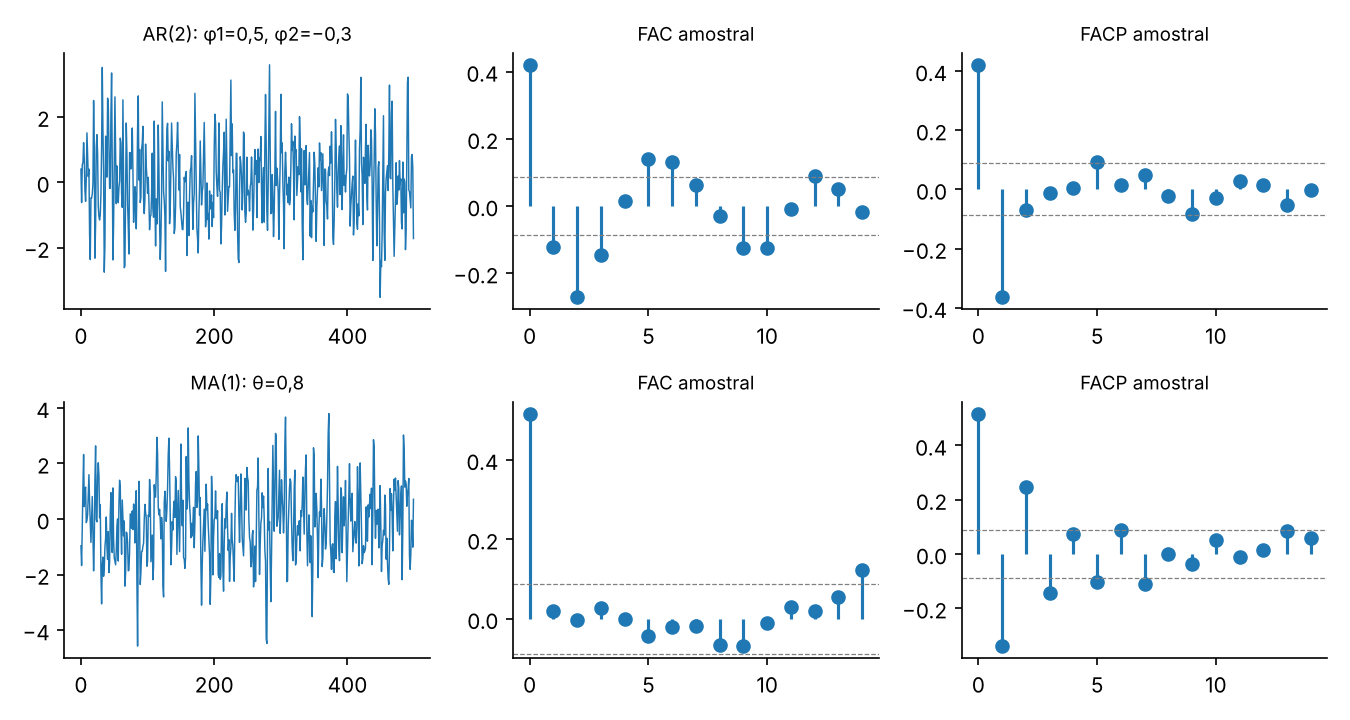
\includegraphics[width=\textwidth]{fig/acf_pacf.png}\\
\small Séries simuladas (500 pontos) e suas FAC e FACP amostrais. Linha de cima: AR(2) ($\phi_1=0{,}5$, $\phi_2=-0{,}3$): a FACP corta em 2. Linha de baixo: MA(1) ($\theta=0{,}8$): a FAC corta em 1. As linhas pontilhadas são as bandas $\pm1{,}96/\sqrt n$.
\end{center}

\begin{atencao}
As bandas $\pm1{,}96/\sqrt n$ valem sob a hipótese de ruído branco. Para uma série que \emph{não} é ruído branco, as bandas corretas (de Bartlett) são mais largas, e em amostras curtas a FAC amostral é viesada para baixo. Interprete os gráficos como pista, não como veredito.
\end{atencao}

\begin{exercicio}
Num AR(1) com $\phi=0{,}6$ e $\sigma^2=1$, calcule $\gamma_0$, $\rho_1$ e $\rho_3$.
\end{exercicio}
\sol{$\gamma_0=\sigma^2/(1-\phi^2)=1/0{,}64=1{,}5625$. $\rho_1=0{,}6$ e $\rho_3=0{,}6^3=0{,}216$.}

\begin{exercicio}
Um MA(1) tem $\theta=-0{,}4$ (convenção positiva). Qual é $\rho_1$? E se a convenção do livro fosse a negativa, com o mesmo número $-0{,}4$ impresso?
\end{exercicio}
\sol{Convenção positiva: $\rho_1=-0{,}4/(1+0{,}16)=-0{,}345$. Convenção negativa, com $\theta=-0{,}4$: $\rho_1=-\theta/(1+\theta^2)=+0{,}345$. O mesmo número com convenções diferentes dá correlações de sinais opostos.}

\chapter{ARMA, ARIMA e a metodologia Box--Jenkins}
\label{cap:arma}

\section{O modelo ARMA e o operador de defasagem}
Com $B y_t=y_{t-1}$, um ARMA($p,q$) escreve-se
\[
\phi(B)\,y_t=\theta(B)\,\varepsilon_t,\qquad \phi(B)=1-\phi_1B-\dots-\phi_pB^p,\quad \theta(B)=1+\theta_1B+\dots+\theta_qB^q.
\]
Duas exigências técnicas: \textbf{estacionariedade} (raízes de $\phi(B)$ fora do círculo unitário) e \textbf{invertibilidade} (raízes de $\theta(B)$ fora do círculo unitário). Esta última garante que o choque $\varepsilon_t$ pode ser recuperado dos dados passados e que o modelo é identificado (vimos que $\theta$ e $1/\theta$ dão a mesma FAC).

\section{ARIMA: o que a letra ``I'' faz}
Se a série tem raiz unitária (passeio aleatório, tendência estocástica), diferencie: $\Delta y_t=y_t-y_{t-1}$. Um ARIMA($p,d,q$) é um ARMA($p,q$) aplicado à série diferenciada $d$ vezes. Quase nunca é necessário $d>2$.

\begin{atencao}[{Superdiferenciação}]
Diferenciar uma série que já é estacionária cria uma raiz unitária no componente MA (o MA fica não invertível). Sintomas: FAC amostral com $\rho_1$ próximo de $-0{,}5$ e variância maior depois de diferenciar. Diferencie apenas o necessário.
\end{atencao}

\section{O ciclo Box--Jenkins em quatro passos}
\begin{enumerate}[leftmargin=1.6em]
\item \textbf{Especificação}: olhe o gráfico da série, decida a transformação (log para variância crescente) e o grau de diferenciação (teste de raiz unitária, capítulo~\ref{cap:ur}). Use FAC e FACP para sugerir candidatos e critérios de informação (AIC, BIC) para compará-los.
\item \textbf{Estimação}: máxima verossimilhança ou mínimos quadrados condicionais.
\item \textbf{Diagnóstico}: os resíduos devem se parecer com ruído branco. Examine a FAC dos resíduos e faça o teste de Ljung--Box.
\item \textbf{Previsão}: apenas com o modelo validado (capítulo~\ref{cap:prev}).
\end{enumerate}

\begin{atencao}[{Armadilha: graus de liberdade do Ljung--Box}]
A estatística $Q=n(n+2)\sum_{k=1}^m\hat\rho_k^2/(n-k)$ é comparada com uma qui-quadrado com $m-p-q$ graus de liberdade, \textbf{não} com $m$, quando se testa resíduos de um ARMA($p,q$) estimado. Usar $m$ torna o teste conservador. Muitos softwares permitem informar $p+q$ para ajustar. Verifique.
\end{atencao}

\begin{intuicao}[{AIC versus BIC}]
Ambos penalizam a complexidade: $\text{AIC}=-2\ln L+2k$ e $\text{BIC}=-2\ln L+k\ln n$. O BIC pune mais e tende a escolher modelos menores e consistentes (encontra o modelo verdadeiro quando ele está entre os candidatos). O AIC tende a favorecer qualidade de previsão. Em caso de divergência, vale olhar os dois e preferir parcimônia.
\end{intuicao}

\section{Sazonalidade}
Para dados com ciclo de período $s$ (12 em dados mensais), usa-se o ARIMA sazonal $(p,d,q)(P,D,Q)_s$: acrescenta-se diferenciação sazonal $(1-B^s)$ e termos AR e MA nas defasagens $s,2s,\dots$ O exemplo clássico é o ``modelo de linhas aéreas'', um ARIMA$(0,1,1)(0,1,1)_{12}$ aplicado ao logaritmo da série. Sazonalidade também pode ser tratada com variáveis indicadoras ou com suavização exponencial (Holt--Winters).

\begin{exercicio}
O modelo $y_t=0{,}5y_{t-1}+\varepsilon_t+0{,}4\varepsilon_{t-1}$ é estacionário e invertível?
\end{exercicio}
\sol{Parte AR: $\phi(B)=1-0{,}5B$, raiz $B=2$, fora do círculo unitário: estacionário. Parte MA: $\theta(B)=1+0{,}4B$, raiz $B=-2{,}5$, fora do círculo: invertível.}

\begin{exercicio}
Uma série tem FAC amostral que decai muito lentamente (0,95; 0,93; 0,91, \dots). O que isso sugere e qual é o próximo passo?
\end{exercicio}
\sol{Autocorrelações muito persistentes são típicas de raiz unitária ou tendência. O próximo passo é aplicar um teste de raiz unitária (ADF, KPSS) e, se confirmada, diferenciar a série antes de identificar o ARMA.}

\chapter{Previsão}
\label{cap:prev}

\section{O melhor previsor}
Para erro quadrático, o melhor previsor de $y_{T+h}$ dado o passado é a esperança condicional $\E(y_{T+h}\mid y_T,y_{T-1},\dots)$ (capítulo~\ref{cap:ec}). Num AR(1) com média $\mu$:
\[
\hat y_{T+h}=\mu+\phi^h(y_T-\mu),\qquad \Var(e_{T+h})=\sigma^2\,\frac{1-\phi^{2h}}{1-\phi^2}.
\]
\begin{intuicao}
Quanto mais longe o horizonte, mais a previsão se aproxima da média de longo prazo, e mais a incerteza se aproxima da variância incondicional $\gamma_0=\sigma^2/(1-\phi^2)$. Para $h$ grande, o modelo não sabe mais do que a média.
\end{intuicao}

\begin{center}
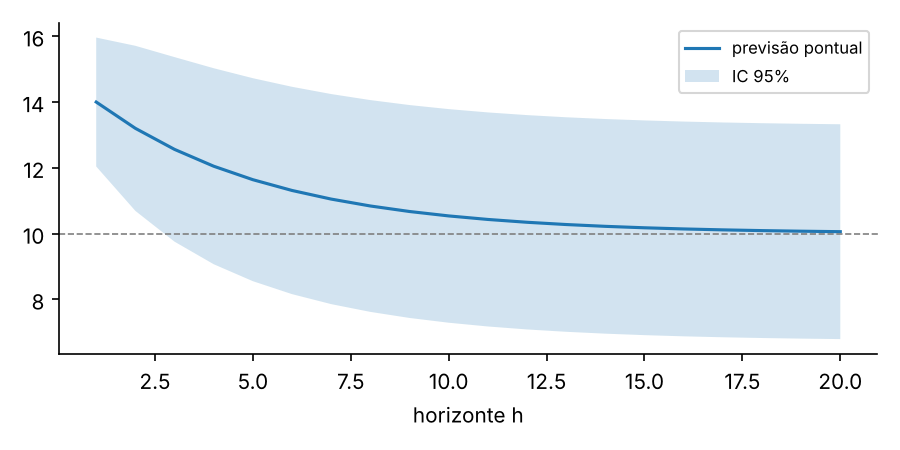
\includegraphics[width=0.75\textwidth]{fig/previsao_ar1.png}\\
\small AR(1) com $\mu=10$, $\phi=0{,}8$, $\sigma=1$ e último desvio $y_T-\mu=5$. A previsão decai para a média e o intervalo alarga e estabiliza.
\end{center}

\begin{simulacao}[{Conferido por simulação: cobertura do intervalo}]
Simulei 4000 séries AR(1) com $\phi=0{,}8$, previ $h=3$ passos à frente e construí o intervalo de 95\%. A cobertura empírica foi $95{,}0\%$. A variância teórica do erro para $h=3$ é $(1-0{,}8^6)/(1-0{,}64)=2{,}0496$, confirmada.
\end{simulacao}

\section{Passeio aleatório e ARIMA}
Num passeio aleatório, $\hat y_{T+h}=y_T$ (previsão ``ingênua'') e $\Var(e_{T+h})=h\sigma^2$. O intervalo cresce sem parar, o que reflete a natureza de choques permanentes. Modelos ARIMA com $d\ge1$ têm essa mesma propriedade, o que é muito diferente de um modelo estacionário.

\begin{atencao}[{Armadilha: intervalos otimistas}]
Os intervalos clássicos tratam os parâmetros estimados como verdadeiros e supõem que o modelo está certo. Com amostras curtas ou escolha de modelo feita com os mesmos dados, a cobertura real costuma ser menor do que a nominal. Em previsão séria, avalie a cobertura fora da amostra.
\end{atencao}

\section{Como avaliar previsões}
\begin{itemize}[leftmargin=1.4em]
\item \textbf{Fora da amostra, sempre.} O ajuste dentro da amostra premia modelos complicados.
\item \textbf{Origem móvel (rolling origin)}: estime até $t$, preveja $t+1,\dots,t+h$, avance a origem e repita.
\item \textbf{Métricas}: MAE e RMSE (mesma unidade da série); MAPE é intuitivo, mas explode se há valores próximos de zero e pune erros positivos e negativos de forma assimétrica; MASE compara com o previsor ingênuo e é comparável entre séries.
\item \textbf{Sempre inclua um \emph{benchmark}}: ingênuo (último valor) ou sazonal ingênuo. Um modelo que não bate o ingênuo não serve.
\end{itemize}

\begin{exercicio}
AR(1) com $\mu=0$, $\phi=0{,}8$, $\sigma^2=1$ e último valor $y_T=5$. Dê a previsão para $h=3$ e o intervalo de 95\%.
\end{exercicio}
\sol{Previsão: $0{,}8^3\times5=0{,}512\times5=2{,}56$. Variância do erro: $2{,}0496$, desvio $1{,}4317$. Intervalo: $2{,}56\pm1{,}96\times1{,}4317=2{,}56\pm2{,}806$, isto é, $[-0{,}25;\,5{,}37]$.}

\begin{exercicio}
Um passeio aleatório tem $\sigma=2$. Qual é o desvio-padrão do erro de previsão a 9 passos?
\end{exercicio}
\sol{$\sqrt{h}\,\sigma=\sqrt9\times2=6$.}

\chapter{Raízes unitárias, regressão espúria e cointegração}
\label{cap:ur}

\section{Tendência determinística versus estocástica}
Duas séries podem ``subir'' por motivos muito diferentes.
\begin{itemize}[leftmargin=1.4em]
\item \textbf{Tendência determinística}: $y_t=a+bt+\text{(estacionário)}$. Os desvios da reta são temporários. Remover a tendência torna a série estacionária.
\item \textbf{Tendência estocástica} (raiz unitária): $y_t=y_{t-1}+\varepsilon_t$. Os choques são permanentes. Remover uma reta \emph{não} resolve; é preciso diferenciar.
\end{itemize}
Tratar uma como se fosse a outra gera erros graves de previsão e de inferência.

\section{Teste de Dickey--Fuller aumentado (ADF)}
Estima-se
\[
\Delta y_t=\alpha+\gamma\,y_{t-1}+\sum_{j=1}^{p}\delta_j\Delta y_{t-j}+e_t,
\]
e testa-se $H_0:\gamma=0$ (há raiz unitária) contra $\gamma<0$ (estacionária). As defasagens extras servem para branquear os resíduos.

\begin{atencao}[{Armadilhas do ADF}]
\begin{itemize}[leftmargin=1.2em]
\item \textbf{A estatística t não segue a distribuição t nem a normal}. Os valores críticos são os de Dickey--Fuller, mais negativos (por exemplo, cerca de $-2{,}86$ a 5\% com constante). Comparar com $-1{,}96$ rejeita demais.
\item \textbf{Os termos determinísticos importam}: sem constante, com constante ou com tendência, os valores críticos mudam e a escolha errada distorce o teste.
\item \textbf{Baixo poder}: o teste tem dificuldade em distinguir raiz unitária de uma raiz próxima de 1 (por exemplo, $\phi=0{,}98$) em amostras moderadas.
\item \textbf{KPSS inverte a hipótese nula} (a nula é estacionariedade). Usar os dois juntos é prática comum: ADF rejeita e KPSS não rejeita $\Rightarrow$ evidência favorável à estacionariedade.
\end{itemize}
\end{atencao}

\begin{simulacao}[{Conferido por simulação}]
Num passeio aleatório de 300 pontos, o ADF deu p-valor $0{,}50$ (não rejeita a raiz unitária, correto). Num ruído branco, o p-valor foi $\approx10^{-29}$ (rejeita fortemente, correto).
\end{simulacao}

\section{Regressão espúria}
Regredir uma série integrada contra outra, independente dela, produz coeficientes ``significativos'' com frequência absurda.

\begin{simulacao}[{Conferido por simulação}]
Simulei 1000 pares de passeios aleatórios \emph{independentes} com 200 observações cada, rodei MQO de um contra o outro e testei a inclinação a 5\%. O teste t rejeitou a hipótese de inclinação zero em \textbf{83,6\%} dos casos, em vez dos 5\% esperados.
\end{simulacao}

\begin{center}
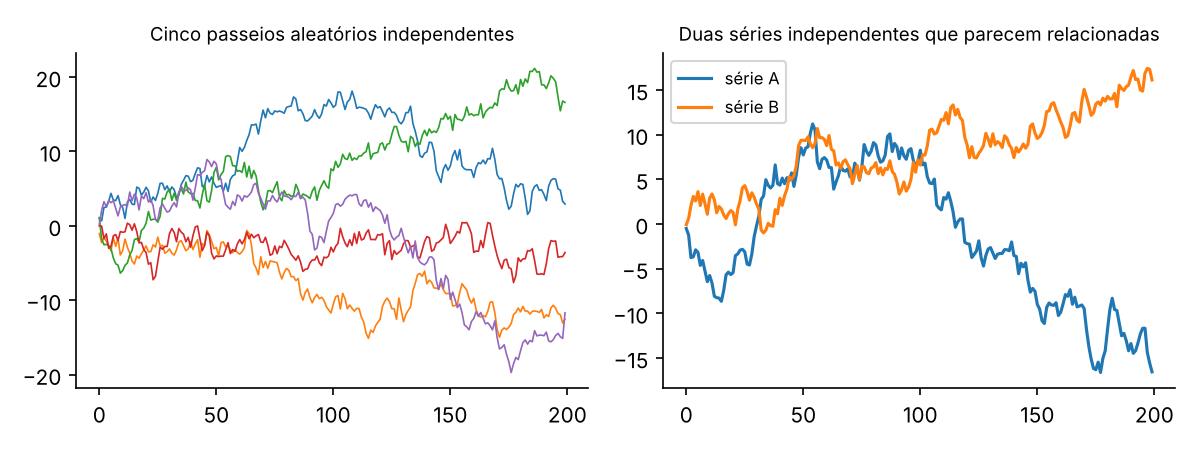
\includegraphics[width=0.9\textwidth]{fig/espuria.png}\\
\small Esquerda: cinco passeios aleatórios independentes, que parecem ter tendências próprias. Direita: duas séries independentes que, por acaso, parecem relacionadas.
\end{center}

\textbf{Regras práticas}: (i) nunca faça MQO em níveis de séries com raiz unitária sem investigar cointegração; (ii) um sinal de alerta clássico é $R^2$ alto com resíduos fortemente autocorrelacionados (estatística de Durbin--Watson próxima de 0); (iii) se não há cointegração, trabalhe com as séries diferenciadas.

\section{Cointegração}
Duas séries $I(1)$ são \textbf{cointegradas} se alguma combinação linear delas é estacionária. Elas podem se afastar no curto prazo, mas uma força as traz de volta (um equilíbrio de longo prazo).

\begin{intuicao}[{O bêbado e o cachorro}]
Dois passeios aleatórios independentes são como um bêbado e um cachorro soltos: cada um vai para onde quer. Cointegração é o bêbado com o cachorro na coleira: ambos vagam sem rumo, mas a distância entre eles é limitada.
\end{intuicao}

\begin{center}
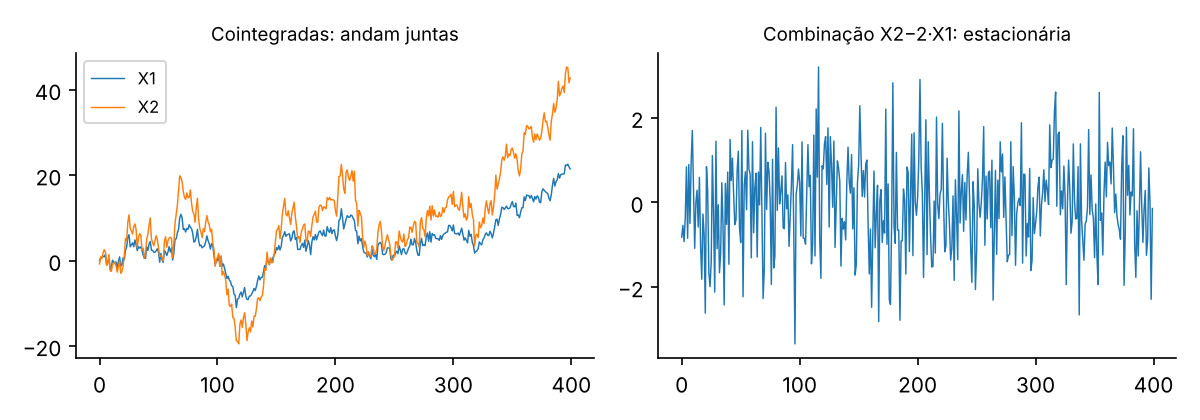
\includegraphics[width=0.9\textwidth]{fig/cointegracao.png}\\
\small $X_1=w+\text{ruído}$ e $X_2=2w+\text{ruído}$, com $w$ um passeio aleatório. Cada série é não estacionária, mas $X_2-2X_1$ é estacionária.
\end{center}

\textbf{Teste de Engle--Granger} (dois passos): (1) regrida uma série na outra; (2) aplique ADF aos resíduos, usando valores críticos \emph{próprios} para resíduos estimados (mais exigentes que os do ADF comum). A alternativa multivariada é o teste de Johansen, que identifica quantas relações de cointegração existem.

\begin{simulacao}[{Conferido por simulação}]
Com 200 observações, repeti 500 vezes. Para pares cointegrados, o teste de Engle--Granger a 5\% rejeitou ``sem cointegração'' em 99,6\% das simulações. Para pares independentes, rejeitou em 7,4\% (um pouco acima dos 5\% nominais em amostras de tamanho moderado, mas muito longe de 84\%).
\end{simulacao}

\textbf{Modelo de correção de erros}: se $y_t$ e $x_t$ são cointegradas, $\Delta y_t=\alpha(y_{t-1}-\beta x_{t-1})+\gamma\Delta x_t+e_t$, com $\alpha<0$ medindo a velocidade com que a economia retorna ao equilíbrio.

\begin{exercicio}
Uma regressão entre duas séries de preços em nível dá $R^2=0{,}95$ e Durbin--Watson de $0{,}1$. O que fazer antes de confiar nesse resultado?
\end{exercicio}
\sol{O padrão ($R^2$ alto, DW muito baixo) é típico de regressão espúria. Teste raiz unitária em cada série; se ambas forem $I(1)$, teste cointegração (Engle--Granger ou Johansen). Sem cointegração, a regressão em níveis não tem interpretação e o correto é modelar as diferenças. Com cointegração, use um modelo de correção de erros.}

\chapter{Vetores autorregressivos (VAR)}
\label{cap:var}

\section{O modelo}
Um VAR($p$) para um vetor de $k$ variáveis é
\[
y_t=c+A_1y_{t-1}+\dots+A_py_{t-p}+u_t,\qquad \E(u_t)=0,\ \ \E(u_tu_t')=\Sigma.
\]
Cada variável é explicada pelas defasagens de \emph{todas} as variáveis, incluindo as suas próprias. A estimação por MQO, equação a equação, é consistente e, quando todas as equações têm os mesmos regressores, equivale à estimação de máxima verossimilhança (sob normalidade).

\textbf{Estabilidade (estacionariedade)}: todos os autovalores da matriz companheira devem ter módulo menor que 1. É o análogo multivariado da condição $|\phi|<1$.

\section{Escolha do número de defasagens}
Estime VARs com $p=1,2,\dots,p_{\max}$ e compare AIC, BIC (ou Hannan--Quinn). Verifique que os resíduos não têm autocorrelação.

\section{Causalidade de Granger}
$x$ \emph{Granger-causa} $y$ se as defasagens de $x$ ajudam a prever $y$ além das defasagens do próprio $y$. Testa-se com um teste F conjunto dos coeficientes de $x$ na equação de $y$.

\begin{atencao}[{Armadilha: Granger não é causalidade}]
É uma noção de \emph{precedência preditiva}. Se um terceiro fator, não incluído, move as duas variáveis com defasagens diferentes, aparece ``causalidade de Granger'' sem causa nenhuma. O nome é enganoso.
\end{atencao}

\begin{simulacao}[{Conferido por simulação}]
Simulei um VAR(1) bivariado com $A=\begin{pmatrix}0{,}5&0{,}2\\0&0{,}4\end{pmatrix}$ ($T=1500$). Estimativa: $\hat A=\begin{pmatrix}0{,}51&0{,}195\\-0{,}005&0{,}399\end{pmatrix}$. Os autovalores de $A$ têm módulos $0{,}5$ e $0{,}4$ (estável). O teste de Granger identificou corretamente: $y_2$ ajuda a prever $y_1$ (p-valor $\approx10^{-15}$) e $y_1$ não ajuda a prever $y_2$ (p-valor $0{,}82$).
\end{simulacao}

\section{Funções de resposta a impulso e decomposição da variância}
A \textbf{resposta a impulso} mostra como cada variável reage, ao longo do tempo, a um choque numa equação. O problema: os erros $u_t$ costumam ser correlacionados entre equações, então ``um choque só em $y_1$'' não existe sem uma hipótese adicional. A solução mais comum é a decomposição de Cholesky, que impõe uma ordem recursiva (a primeira variável afeta as demais no mesmo período, mas não o contrário).

\begin{atencao}
\textbf{A ordem das variáveis na decomposição de Cholesky muda os resultados} quando os erros são correlacionados. Isso é uma escolha de identificação, e precisa ser justificada economicamente, não decidida por conveniência. A decomposição da variância do erro de previsão (FEVD) herda o mesmo problema.
\end{atencao}

\begin{exercicio}
Um VAR(1) tem $A=\begin{pmatrix}0{,}6&0{,}3\\0{,}2&0{,}5\end{pmatrix}$. Ele é estável?
\end{exercicio}
\sol{Autovalores: $\lambda^2-(0{,}6+0{,}5)\lambda+(0{,}6\cdot0{,}5-0{,}3\cdot0{,}2)=\lambda^2-1{,}1\lambda+0{,}24=0$. Então $\lambda=(1{,}1\pm\sqrt{1{,}21-0{,}96})/2=(1{,}1\pm0{,}5)/2$, isto é, $0{,}8$ e $0{,}3$. Ambos têm módulo menor que 1: o VAR é estável.}

\chapter{Volatilidade: ARCH e GARCH}
\label{cap:garch}

\section{O problema}
Retornos financeiros têm três traços estáveis: (i) quase sem autocorrelação, (ii) \emph{quadrados} dos retornos fortemente autocorrelacionados (a volatilidade vem em ondas: calmaria, turbulência), (iii) caudas mais pesadas do que as de uma normal. Um ARMA clássico supõe variância constante e não captura nada disso.

\section{ARCH(1) e GARCH(1,1)}
Escreva o retorno (já sem média) como $r_t=\sigma_t z_t$, com $z_t$ i.i.d. de média 0 e variância 1. No \textbf{GARCH(1,1)}:
\[
\sigma_t^2=\omega+\alpha\,r_{t-1}^2+\beta\,\sigma_{t-1}^2,\qquad \omega>0,\ \alpha,\beta\ge0.
\]
\begin{itemize}[leftmargin=1.4em]
\item O ARCH(1) é o caso $\beta=0$: a volatilidade de hoje depende só do choque de ontem.
\item \textbf{Estacionariedade}: $\alpha+\beta<1$. Variância incondicional: $\omega/(1-\alpha-\beta)$.
\item $\alpha+\beta$ mede a \textbf{persistência}. Valores próximos de 1 (como 0{,}97) são típicos em dados reais.
\item A curtose (de $r_t$) é maior do que 3 mesmo com $z_t$ normal.
\end{itemize}

\begin{simulacao}[{Conferido por simulação}]
Com $\omega=0{,}1$, $\alpha=0{,}1$, $\beta=0{,}85$ e uma simulação longa (400 mil pontos): variância $2{,}009$ (teoria: $0{,}1/0{,}05=2$); curtose $3{,}774$ (teoria: $3{,}774$); autocorrelação de $r_t^2$ no lag 1: $0{,}177$ (teoria: $0{,}179$). A autocorrelação de $r_t$ ficou próxima de zero ($0{,}04$ numa amostra de 2000 pontos), mas a de $r_t^2$ foi $0{,}15$. Ruído branco nos retornos, dependência forte na volatilidade.
\end{simulacao}

\begin{center}
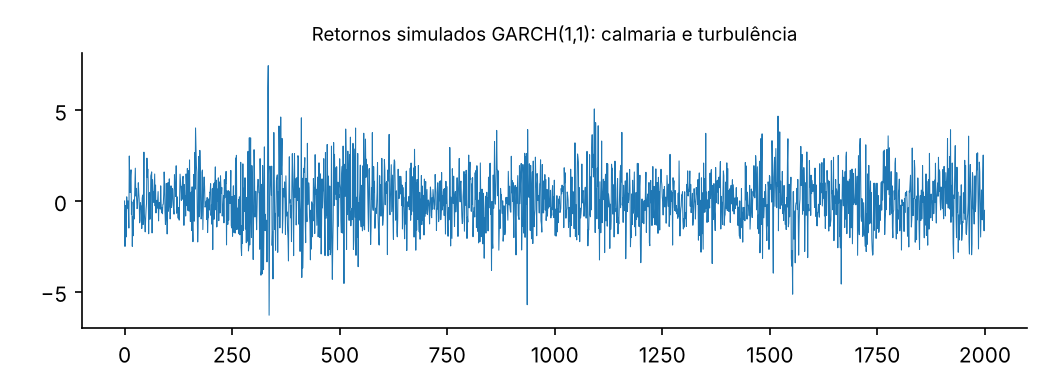
\includegraphics[width=0.9\textwidth]{fig/garch.png}
\end{center}

\begin{simulacao}[{Estimação: parâmetros individuais são difíceis}]
Ajustando um GARCH(1,1) a 2000 pontos simulados, obtive $\hat\omega=0{,}054$, $\hat\alpha=0{,}086$ e $\hat\beta=0{,}890$, contra os verdadeiros $0{,}1$; $0{,}1$; $0{,}85$. Os parâmetros individuais erraram bastante, mas a combinação que importa ficou próxima: persistência estimada $0{,}976$ (verdadeira $0{,}95$) e variância incondicional $0{,}054/0{,}024\approx2{,}26$ (verdadeira $2{,}0$). Em modelos muito persistentes, $\omega$, $\alpha$ e $\beta$ ficam fortemente correlacionados na estimação.
\end{simulacao}

\begin{atencao}
\begin{itemize}[leftmargin=1.2em]
\item \textbf{Não aplique ARCH a uma série com raiz unitária ou tendência}; trabalhe com retornos (diferenças de logaritmos).
\item \textbf{O GARCH simétrico não distingue notícias boas de ruins.} Para o efeito alavancagem (quedas aumentam mais a volatilidade do que altas), use GJR-GARCH ou EGARCH.
\item \textbf{Escolher $z_t$ normal subestima caudas}; muitos usam $t$ de Student.
\end{itemize}
\end{atencao}

\begin{exercicio}
GARCH(1,1) com $\omega=0{,}2$, $\alpha=0{,}1$, $\beta=0{,}8$. Calcule a variância incondicional e a previsão de $\sigma^2_{t+1}$ dado $r_t^2=4$ e $\sigma_t^2=3$.
\end{exercicio}
\sol{Variância incondicional: $0{,}2/(1-0{,}9)=2$. Previsão: $\sigma^2_{t+1}=0{,}2+0{,}1\times4+0{,}8\times3=0{,}2+0{,}4+2{,}4=3{,}0$.}

\begin{exercicio}
Por que $\alpha+\beta=1$ cria problemas, e como se chama esse caso?
\end{exercicio}
\sol{Com $\alpha+\beta=1$ a variância incondicional não existe (o denominador é zero) e choques de volatilidade nunca se dissipam. É o IGARCH. A previsão da volatilidade futura deixa de reverter para uma média de longo prazo.}

\chapter{Aprendizado de máquina para séries temporais}
\label{cap:ml}

\section{O que muda quando os dados têm ordem}
Os métodos de aprendizado de máquina (florestas aleatórias, \emph{boosting}, redes neurais) foram desenhados, em sua maioria, para observações independentes. Em séries temporais, três cuidados são obrigatórios.

\subsection{Validação cruzada que respeita o tempo}
A validação cruzada aleatória (\emph{k-fold} com embaralhamento) mistura passado e futuro. Como observações vizinhas são parecidas, o modelo ``vê'' pontos quase idênticos ao que vai prever. Isso vaza informação e subestima o erro.

\begin{simulacao}[{Conferido por simulação: vazamento na validação}]
Série AR(1) muito persistente ($\phi=0{,}98$, ruído de desvio-padrão 1), floresta aleatória com 5 defasagens como variáveis explicativas. RMSE com validação cruzada aleatória: $1{,}08$. RMSE com validação temporal (treino no passado, teste no futuro): $1{,}49$. O ruído irredutível é $1{,}0$. O procedimento aleatório parece quase perfeito. O temporal mostra o desempenho real, bem pior. A diferença é puro vazamento.
\end{simulacao}

Use sempre \textbf{validação com janela móvel ou expansiva} (origem móvel, como no capítulo~\ref{cap:prev}), e, quando houver sobreposição entre janelas, deixe uma folga (\emph{gap}) entre treino e teste.

\subsection{Árvores não extrapolam}
Uma árvore (e uma floresta) prevê médias de observações já vistas. Se a série tem tendência e o futuro sai do intervalo do treino, ela fica ``presa'' no último patamar.

\begin{center}
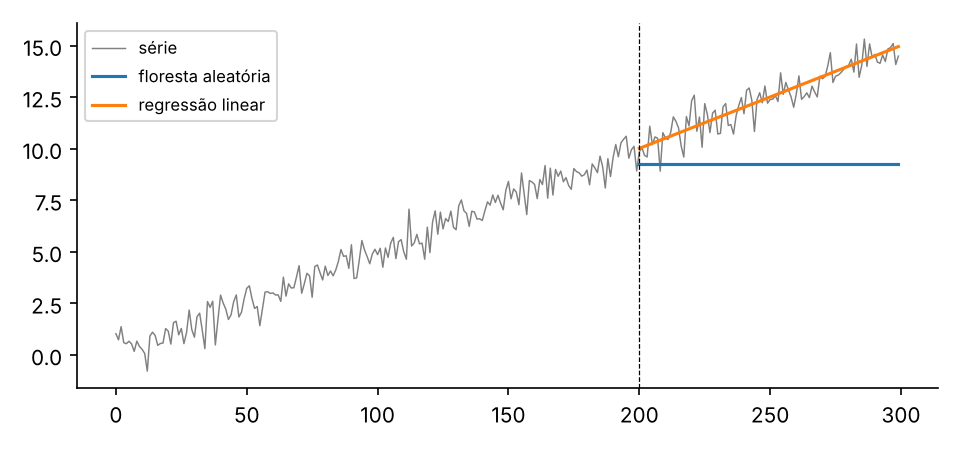
\includegraphics[width=0.75\textwidth]{fig/rf_extrapola.png}\\
\small Série com tendência linear. A floresta aleatória, treinada até $t=200$, prevê um patamar plano; a regressão linear continua a tendência.
\end{center}

\begin{simulacao}
No ponto $t=299$, a floresta previu $9{,}27$, e o valor da tendência é $14{,}95$.
\end{simulacao}

Soluções: diferenciar ou remover a tendência antes de ajustar, modelar a variação em vez do nível, ou usar um modelo híbrido (tendência linear mais floresta nos resíduos).

\subsection{Construção das variáveis explicativas}
Para transformar previsão em problema de regressão: use defasagens ($y_{t-1},\dots,y_{t-p}$), médias móveis, variáveis de calendário (mês, dia da semana, feriados) e regressores externos. Qualquer estatística construída com dados do futuro (por exemplo, normalizar com a média da série inteira) é vazamento.

\section{Duas famílias úteis}
\begin{itemize}[leftmargin=1.4em]
\item \textbf{Modelos globais}: em vez de ajustar um modelo por série, treina-se um único modelo (por exemplo, uma rede neural recorrente ou um \emph{boosting}) com milhares de séries. Ajuda quando cada série é curta ou ruidosa. É a ideia central do tutorial de Faloutsos e coautores sobre previsão em larga escala.
\item \textbf{Classificação de séries}: o problema não é prever, mas atribuir um rótulo a uma série inteira (por exemplo, normal versus anomalia num eletrocardiograma). É o foco do pacote \texttt{pyts}, que oferece técnicas como \emph{dynamic time warping}, \emph{shapelets} e representações em imagem. Não confunda com previsão.
\end{itemize}

\begin{atencao}[{Armadilhas}]
\begin{itemize}[leftmargin=1.2em]
\item \textbf{Sempre compare com o previsor ingênuo e com um ARIMA/ETS}. Muitos resultados deslumbrantes de redes profundas desaparecem diante de um \emph{benchmark} simples.
\item \textbf{Intervalos de previsão}: modelos de ML dão previsões pontuais. Para incerteza, use regressão por quantis, \emph{conformal prediction} ou simulação.
\item \textbf{Hiperparâmetros ajustados nos dados de teste}: o teste deve ser tocado uma única vez.
\end{itemize}
\end{atencao}

\begin{exercicio}
Por que embaralhar as observações antes de dividir em treino e teste é um erro numa série temporal?
\end{exercicio}
\sol{Porque faz o modelo treinar com observações do futuro e testar no passado, e porque observações adjacentes são fortemente dependentes: pontos de teste têm quase-duplicatas no treino. O erro estimado fica irrealisticamente baixo. O teste correto respeita a ordem cronológica.}

\part{Consulta rápida}
\chapter{Cola de armadilhas e convenções}
\label{cap:cola}

Esta lista reúne os pontos em que livros, softwares e intuições costumam divergir. Cada item aparece no capítulo indicado.

\begin{center}
\small
\begin{longtable}{p{0.5cm}p{6.6cm}p{6.5cm}}
\toprule
\textbf{\#} & \textbf{Armadilha} & \textbf{Conduta correta} \\
\midrule
\endhead
1 & Tomar $\E(u\mid x)=0$ como necessário para consistência do MQO (cap.~\ref{cap:mqo}) & Basta $\E(x'u)=0$. A hipótese condicional é necessária para a interpretação como esperança condicional e para resultados de amostra finita. \\
2 & Corrigir heterocedasticidade só depois de ``testar'' (cap.~\ref{cap:mqo}) & Reporte erros robustos diretamente: valem nos dois casos. \\
3 & Esquecer que erro robusto a heterocedasticidade não corrige autocorrelação (cap.~\ref{cap:mqo}, \ref{cap:painel}) & HAC em séries, erros agrupados em painéis. \\
4 & Interpretar viés de variável omitida sem checar os dois sinais (cap.~\ref{cap:omit}) & O viés é $\beta_2\delta_1$. O sinal é o produto dos dois. \\
5 & Esperar que erro de medida sempre atenue (cap.~\ref{cap:omit}) & Só vale para erro clássico num regressor. Com vários regressores ou erro não clássico, o efeito é incerto. \\
6 & Rodar o 2º estágio de VI à mão (cap.~\ref{cap:vi}) & Use um comando de MQ2E, que corrige os erros-padrão. \\
7 & Confiar na regra ``F $>10$'' como garantia (cap.~\ref{cap:vi}) & É um mínimo. Reporte também intervalos robustos a instrumentos fracos. \\
8 & Usar Hausman clássico com erros robustos (cap.~\ref{cap:painel}) & Use a versão de Mundlak com erros agrupados. \\
9 & Esquecer que efeitos fixos exigem exogeneidade estrita (cap.~\ref{cap:painel}) & Com defasagem da dependente ou \emph{feedback}, use painel dinâmico (GMM). \\
10 & Copiar fórmula de MA de um livro e coeficiente de um software sem checar o sinal (cap.~\ref{cap:est}) & Cryer--Chan e Mills: $\varepsilon_t-\theta\varepsilon_{t-1}$. Hamilton, R, \texttt{statsmodels}: $\varepsilon_t+\theta\varepsilon_{t-1}$. \\
11 & Usar bandas $\pm1{,}96/\sqrt n$ como veredito (cap.~\ref{cap:est}) & Valem sob ruído branco. Para outras séries, as bandas são mais largas. \\
12 & Ljung--Box com $m$ graus de liberdade em resíduos de ARMA (cap.~\ref{cap:arma}) & Use $m-p-q$. \\
13 & Comparar a estatística ADF com $-1{,}96$ (cap.~\ref{cap:ur}) & Use valores críticos de Dickey--Fuller (cerca de $-2{,}86$ a 5\% com constante). \\
14 & Regredir séries integradas em nível (cap.~\ref{cap:ur}) & Teste cointegração. Se não houver, diferencie. \\
15 & Supor que o intervalo de previsão tem cobertura exata (cap.~\ref{cap:prev}) & Ele ignora incerteza dos parâmetros e do modelo. Avalie a cobertura fora da amostra. \\
16 & Ler Granger como causalidade (cap.~\ref{cap:var}) & É precedência preditiva. \\
17 & Ignorar a ordem de Cholesky nas respostas a impulso (cap.~\ref{cap:var}) & A ordem é uma hipótese de identificação e muda os resultados. \\
18 & Interpretar $\omega$, $\alpha$, $\beta$ isoladamente em GARCH persistente (cap.~\ref{cap:garch}) & Olhe a persistência $\alpha+\beta$ e a variância incondicional. \\
19 & Validação cruzada aleatória em séries (cap.~\ref{cap:ml}) & Validação temporal, com origem móvel. \\
20 & Esperar que árvores extrapolem tendência (cap.~\ref{cap:ml}) & Remova a tendência ou use modelo híbrido. \\
\bottomrule
\end{longtable}
\end{center}

\section*{Roteiro de estudo sugerido}
\begin{enumerate}[leftmargin=1.6em]
\item Capítulos~\ref{cap:ec} a~\ref{cap:mqo}: faça todos os exercícios, à mão.
\item Capítulos~\ref{cap:omit} e~\ref{cap:vi}: replique as simulações em Python ou R, mudando os parâmetros, até prever o resultado antes de rodar.
\item Capítulo~\ref{cap:painel}: monte um painel simulado com $c_i$ correlacionado e descorrelacionado e compare os estimadores.
\item Capítulos~\ref{cap:est} a~\ref{cap:prev}: ajuste ARIMA a uma série real, faça o diagnóstico e a avaliação com origem móvel.
\item Capítulos~\ref{cap:ur} a~\ref{cap:garch}: teste raiz unitária e cointegração em pares de séries de preços; estime um GARCH em retornos diários.
\item Capítulo~\ref{cap:ml}: reproduza o vazamento da validação cruzada e depois resolva com validação temporal.
\end{enumerate}

\end{document}
